%
% Anlagendesign
%
% @version 1.0
% @author dmayer
% @created 29. Dezember 2015

\setchapterpreamble[o]{%
\dictum[--- \textsc{Charles Eames}]{\Gun Design is the appropriate combination of materials in order to solve a problem. \Gob}}
\renewcommand{\chapterheadstartvskip}{\vspace*{2cm}}

\chapter{Anlagendesign}
\label{chap:anlagendesign}

\renewcommand{\chapterheadstartvskip}{\vspace*{-0.5cm}}

Ziel dieses Kapitel ist es, eine Anlage zur Raumtemperaturregelung für den Betrieb mit Modellprädiktiver Regelung zu konzipieren, zu konkretisieren und im letzten Schritt umzusetzen. Dazu werden zunächst die Anforderungen an die Anlage analysiert und weiterhin die Vorgaben und Rahmenbedingungen zur Anlage von Seiten der Hochschule Karlsruhe spezifiziert und ausgeführt. Daraus wird eine Idee abgeleitet, die anschließend zu einem Konzept weiterentwickelt und in ein konkretes Anlagendesign umgesetzt wird. Dabei werden die einzelnen Anlagenteile und deren Funktionsweisen näher beschrieben und auf die realen Einsatzbedingungen ausgelegt. Abschließend wird die Installation und dabei aufgetretenen Besonderheiten der Anlage beschrieben.

\section{Analyse der Anforderungen und Rahmenbedingungen}
\label{sec:anforderungen}

Um die Anforderungen an eine MPC-fähige Anlage zu bestimmen, wird zunächst der Zweck und die Einsatzziele der Anlage untersucht. In Kapitel \ref{sec:motivation} wurde bereits darauf hingewiesen, dass es die Vorgabe von Seiten der Hochschule war, die Einsatzziele in Einklang zu der bisherigen Forschung zu bringen und komplementär zu wählen. Daher wurden im Dialog mit den Projektverantwortlichen\footnote{In Person von Herrn \textsc{Adrian Bürger} und \textsc{Markus Bohlayer}} für die Forschung im Bereich solarer Anwendungen an der Hochschule Karlsruhe gemeinsam konkrete Einsatzziele der Anlage erarbeitet. Als Ergebnis wurden die folgenden, konkreten Ziele vereinbart:
 
\begin{itemize}
	\item Die Einarbeitung in die Thematiken Modellbildung, Kommunikation von technischen Systemen und Modellprädiktive Regelung soll durch eine praktisches Anwendung unterstützt werden.
	\item Es soll Know-how im Bereich der Kommunikation von technischen Systemen aufgebaut werden, insbesondere im Umgang mit der Software, der Hardware und zahlreichen Schnittstellen.
	\item Die Anlage soll eine hohe Funktionalität, also möglichst wartungsarm, und eine hohe Robustheit gegenüber Fehlern und Beschädigungen besitzen, da bei der Einarbeitung eine erhöhte Wahrscheinlichkeit der Fehlbedienung besteht und Schäden dadurch vermieden werden sollen.
	\item Es soll ein Vergleich verschiedener Regelungsmethodiken beim Einsatz von Modellprädiktiver Regelung ermöglicht werden.
	\item Außerdem soll ein Vergleich von Ergebnissen bei der Variation von Steuerungsparametern sowie beim Einsatz verschiedener Steuerungs- und Regelungsalgorithmen ermöglicht werden.
	\item Des Weiteren soll die Anlage möglichst flexibel ansteuerbar und erweiterbar sein, damit der Grad der Komplexität anpassbar ist und die Anlage um weitere Funktionen oder Features ergänzt werden kann.
	\item Der temperaturerhöhende Effekt der Sonneneinstrahlung auf die Raumtemperatur soll untersucht werden können.
	\item Im Rahmen der Anwendungsforschung soll der Raum zur Temperaturregelung möglichst nahe an der Realität sein, also Störgrößen beinhalten und nicht ungenutzt beziehungsweise leerstehend sein.
\end{itemize}

Zusammenfassend wurde festgehalten, dass die Anlage als Forschungsumgebung für Entwicklungs-, Test- und Anwendungszwecke von verschiedenen Steuerungen und Regelungen dienen soll.

Weiterhin wurden von Seiten der Hochschule Karlsruhe\footnote{In Person von Frau Professor \textsc{Angelika Altmann-Dieses}, Herrn Professor \textsc{Marco Braun} und Herrn \textsc{Adrian Bürger}} Rahmenbedingungen definiert, die im Folgenden zusammengefasst sind:

\begin{itemize}
	\item Der Raum K004a im K Gebäude der Hochschule Karlsruhe wird zur Installation der Anlage und Einrichtung der Forschungsumgebung zur Verfügung gestellt.
	\item Die Installation der Anlage muss mit minimalem baulichem und finanziellem Aufwand zu realisieren sein.
	\item Für die Kommunikation innerhalb der Anlage soll die Modbus Kommunikationstechnologie mit mindestens zwei verschiedenen Übertragungsprotokollen genutzt werden.
	\item Die Modellprädiktive Regelung soll mit Hilfe der Plattform JModelica.org erfolgen.
\end{itemize}

Diese Einsatzziele und Rahmenbedingungen definieren implizit Anforderungen an eine Anlage, welche im Nachfolgenden explizit ausgeführt werden und aus Gründen der Übersichtlichkeit die wichtigsten in Tabelle \ref{tab:anforderungen_umgebung} zusammengefasst sind.

%Here we go

\begin{table}[H]
\centering
\small
\renewcommand{\arraystretch}{1.3}
\begin{tabularx}{1\textwidth}{m{0.35\textwidth}m{0.58\textwidth}}

\toprule

\textbf{Einsatzziele \&} & \multirow{2}{\hsize}{\textbf{Anforderungen}} \\ 
\textbf{Rahmenbedingungen} & \\

\cmidrule[0.5pt](r{0.25em}){1-1} 
\cmidrule[0.5pt](l{0.25em}){2-2}

Raum K004a als Umgebung  & \multirow{3}{\hsize}{
\begin{minipage}[t]{0.57\textwidth}
\begin{itemize}[itemsep=0pt,topsep=0pt,leftmargin=5mm]
	\item Die Anpassung der Anlage an K004a.
	\item Die Nutzung bestehender Heizkörper anstatt einer Klimatisierung des Raumes. 
	\item Die Beschränkung auf eine minimale Funktionalität und Anzahl der einzelnen Komponenten. 
\end{itemize}
\end{minipage}
}
 \\
	
\cmidrule[0.1pt](lr{2em}){1-1} 
Minimaler baulicher Aufwand & \\

\cmidrule[0.1pt](lr{2em}){1-1} 
Minimaler finanzieller \newline Aufwand &\\ 



\cmidrule[0.5pt](r{0.25em}){1-1} 
\cmidrule[0.5pt](l{0.25em}){2-2}

\addlinespace[4mm] Modellprädiktive Regelung mit JModelica.org und CasADi \newline & \multirow{3}{\hsize}{
\begin{minipage}[t]{0.57\textwidth}
\begin{itemize}[itemsep=0pt,topsep=0pt,leftmargin=5mm]
\item Die Modellbildung erfolgt in Modelica.
\item Die Kompatibilität aller Softwareschnittstellen ist in Python durch verschiedene, bereits bestehende Pakete gegeben.
\item Die Kommunikation der Anlage erfolgt gemäß den Modbus~RTU und TCP Protokollspezifikationen.
\item Über Modbus~TCP erfolgt die Ansteuerung der Anlage innerhalb eines gesamten lokalen Netzwerks.
\end{itemize}
\end{minipage}
}  \\

\cmidrule[0.1pt](lr{2em}){1-1}
\addlinespace[4mm] Einsatz der Modbus \newline Kommunikationstechnologie \newline 	& 		\\

\cmidrule[0.1pt](lr{2em}){1-1}
\addlinespace[4mm] Flexible Ansteuerung der Anlage \newline & \\

\cmidrule[0.5pt](r{0.25em}){1-1} 
\cmidrule[0.5pt](l{0.25em}){2-2}

Einarbeitung in die Thematiken:
\begin{minipage}[t]{0.34\textwidth}
\begin{itemize}[itemsep=0pt,topsep=0pt,leftmargin=4mm]
	\item Modellbildung,
	\item Kommunikation technischer \newline Systeme,
	\item und Modellprädiktive \newline Regelung.
\end{itemize}
\end{minipage}
 	& \multirow{2}{\hsize}{
\begin{minipage}[t]{0.57\textwidth}
\begin{itemize}[itemsep=0pt,topsep=0pt,leftmargin=5mm]
	\item Komplexität ist notwendig, darf jedoch nicht zu hoch sein.
	\item Es sind möglichst wenige thematische Überschneidungen erwünscht, daher wird eine klare Struktur mit möglichst scharfer Trennung benötigt.
\end{itemize}
\end{minipage}
}  \\

\cmidrule[0.1pt](lr{2em}){1-1} 

Know-how für Kommunikation \newline technischer Systeme 	&		\\

\cmidrule[0.5pt](r{0.25em}){1-1} 
\cmidrule[0.5pt](l{0.25em}){2-2}

Vergleich von Ergebnissen durch:
\begin{minipage}[t]{0.34\textwidth}
\begin{itemize}[itemsep=0pt,topsep=1pt,leftmargin=4mm]
	\item die Variation von \newline Steuerungsparametern,
	\item den Einsatz verschiedener \newline Regelungsmethodiken,
	\item und den Einsatz \newline verschiedener Algorithmen.
\end{itemize}
\end{minipage}

& \multirow{3}{\hsize}{
\begin{minipage}[t]{0.57\textwidth}
\begin{itemize}[itemsep=0pt,topsep=0pt,leftmargin=5mm]
\item Die Reaktion des Systems muss schnell messbar sowie günstig und einfach zu erfassen sein.
\item Der Einsatz von robusten und einfachen Bauteile.
\item Nutzung eines wartungsarmen Systems.
\item Eine einfache, modulare Erweiterbarkeit des Systems für weitere Schritte muss gegeben sein.
\end{itemize}
\end{minipage}
}  \\

\cmidrule[0.1pt](lr{2em}){1-1} 

Hohe Funktionalität und \newline Robustheit & \\

\cmidrule[0.1pt](lr{2em}){1-1} 

Erweiterbarkeit der Anlage
 &  \\

\bottomrule
\end{tabularx}
\caption{Umsetzung der Ziele in Anforderungen der Anlage}
\label{tab:anforderungen_umgebung}
\end{table}

Die grundlegendste Anforderung an die Planung ist die Anpassung an die räumliche Lage und den Gegebenheiten des Raumes K004a, welche in \ref{fig:skizzek004a} skizziert sind. 
Der Raum befindet auf dem Campus der Hochschule Karlsruhe an der südwestlichen Ecke des K Gebäudes im Erdgeschoss. Die südliche und westliche Außenwand teilt sich der Raum mit der Außenumgebung. Die östliche und nördliche Innenwand sowie die Decke und der Boden des Raumes teilt der Raum hingegen mit angrenzenden Räumen im K Gebäude. Des Weiteren ist in der südlichen Außenwand eine Fensterfront mit Jalousien zur Verschattung eingebaut und direkt darunter ist ein Heizkörper installiert.

\begin{figure}
\centering
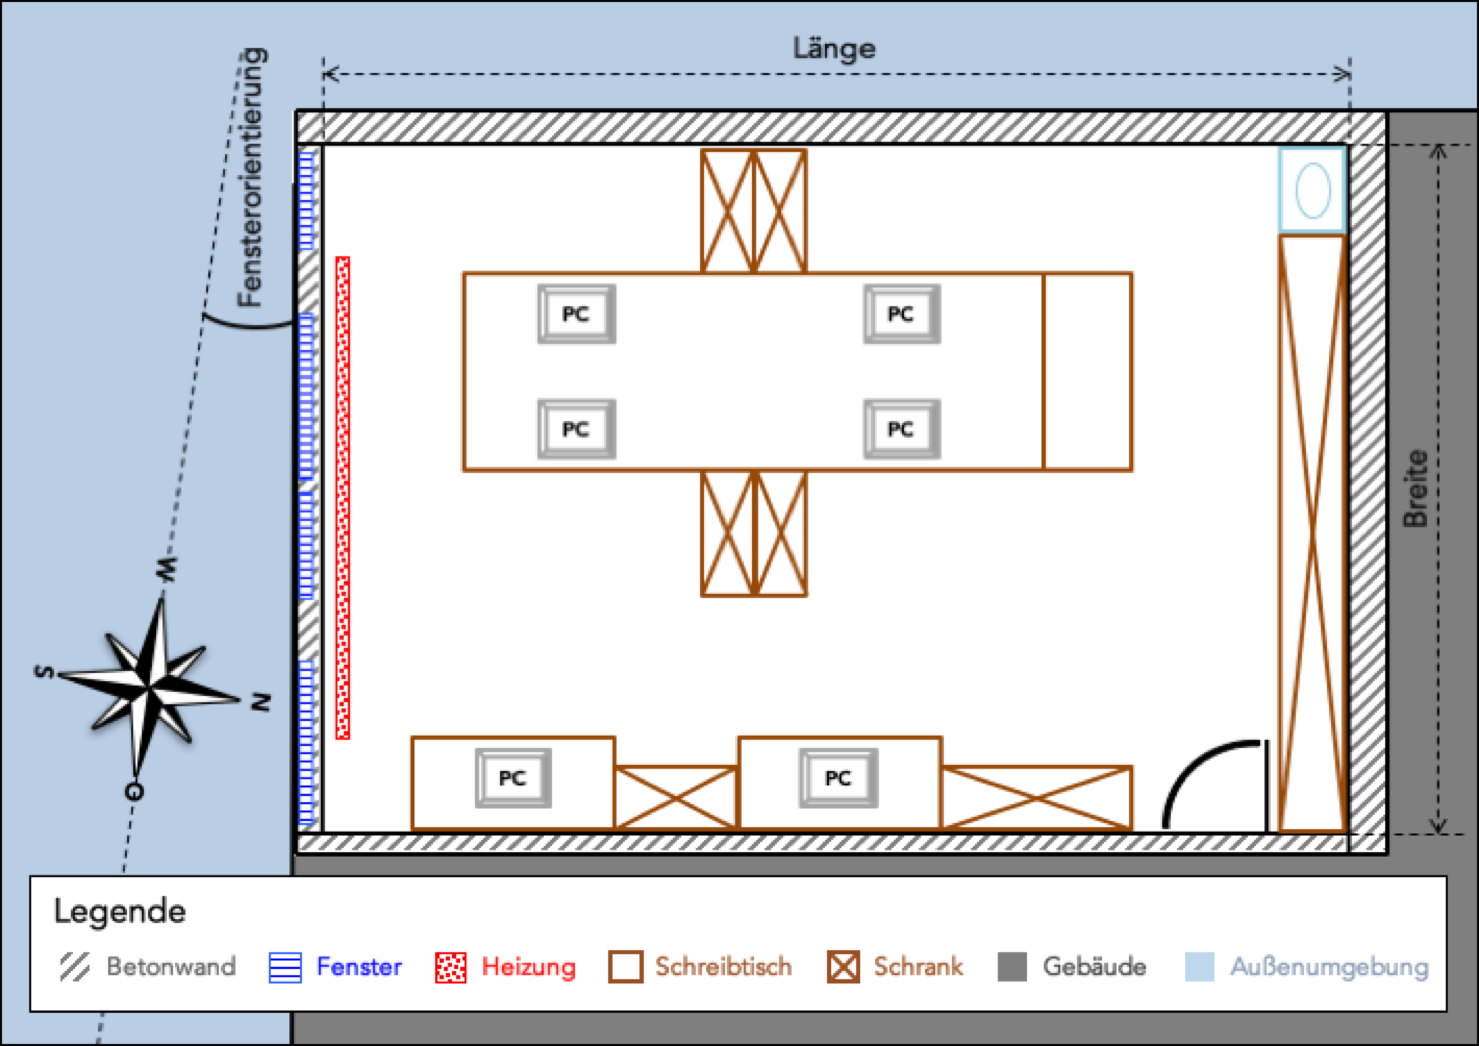
\includegraphics[width=\textwidth]{abbildungen/20160102_k004a}
\caption[Raumskizze K004A vom K Gebäude der Hochschule Karlsruhe -- Technik und Wirtschaft]{Raumskizze K004A vom K Gebäude der Hochschule Karlsruhe -- Technik und Wirtschaft}
\label{fig:skizzek004a}
\end{figure}

Dadurch werden bereits zwei wichtige Anforderungen erfüllt, denn durch die Fensterfront an der Südseite des Raumes kann der Einfluss der Sonneneinstrahlung auf die Raumtemperatur untersucht werden und der vorhandene Heizkörper kann in die Anlage integriert werden, um einen minimalen baulichen und finanziellen Aufwand sicherzustellen.
Damit wird auch eine Klimatisierung des Raumes zur Temperaturregelung zunächst ausgeschlossen, weil diese mit einem erheblichen finanziellen und baulichen Aufwand verbunden ist. Da es jedoch eine weitere Anforderung ist, Erweiterungen der Anlage explizit zu berücksichtigen und ermöglichen, wird bei der Planung darauf geachtet, dass eine Klimatisierung und Ansteuerung der Jalousie für weitere Schritte möglich sein soll

Weiterhin dient der Raum als Büro für wissenschaftliche Mitarbeiter, weshalb sich neben sechs Computerarbeitsplätzen auch Büromobiliar, bestehend aus Schränken und Schreibtischen, darin befindet.

Damit wird auch der Forderung nach einer anwendungsnahen Umgebung sorge getragen, denn durch die Rechner und Mitarbeiter sind nicht vorhersehbar/ bedingt steuerbare parameter größen innerhalb der Anlage.

Eine weitere restriktive Vorgabe ist, dass die Modellprädiktive Regelung mit Hilfe der Plattform JModelica.org und erfolgen soll. JModelica.rog ist eine Umgebung zur Simulation und Optimierung von dynamischen Systemen \cite[S.~1f.]{jmod15} und besitzt eine eigene Klasse für Modellprädiktive Regelung. Der Compiler übersetzt Modelica Modelle direkt in OptimizationProblem Objekte, welche eine symbolische Repräsentation des Optimierungsproblems dass mit CasADi \cite{An13} zur Optimierung benutzt werden kann \cite[S.~12]{jmod15}. Besitzt eine Python Schnittstelle
Daher die Anforderung an die Modellbildung, da das Modell ebenfalls ein Teil der Anlage für MPC ist, in Kapitel \ref{chap:modellbildung}, dass die Modellbildung in Modelica stattfindet.
CasADi wiederum ist eine Open-Source Software für numerische Optimierung allgemein und für die Optimalsteuerung von nichtlinearen Gleichungssystemen. CasADi eignet sich aufgrund seiner effizienten Ableitungserzeugung durch Algorithmische Differentation besonders für Optimierungszwecke \cite[S.~5f.]{casadi}. und besitzte eine Python Schnittstelle

Die Optimalsteuerung stellt in diesem Fall den begrenzenden Faktor dar, da die Optimierungsumgebund CasADi für dynamische Systeme nur unter JModelica.org läuft. Daher wird darauf aufbauend das benötigte Modell für die MPC in Modelica gebildet unter Berücksichtigung der Restriktionen bezüglich JModelica. Die gemeinsame Schnittstelle beider ist Python, übder die damit auch die Kommunikation mit den Hardwarekomponenten der Heizungstseurung erfolgen muss/soll.

Des Weiteren soll die Kommunikation mit Hilfe der Modbus Kommunikationstechnologie stattfinden, da die große Anlage der HsKa einfacher in Betrieb genommen werden kann. Um weitere Erfahrungen und das Know-how ein wenig breiter werden die beiden Modbus Protokolle RTU und TCP Anwendung finden und über verschiedene elektrische Schnittstellen genutzt werden. Das Modbus Protokoll wurde in verschiedenen Python Paketen bereits umgesetzt.

Damit die Einarbeitung in die Themengebiete Modellbildung, Modellprädiktive Regelung und Kommunikation technischer Systeme vereinfacht wird, sollte die Anlage möglichst wenig Komplexität aufweisen. Damit die Zusammenhänge in den einzelnen und Wechselwirkungen zwischen den Fachgebieten und Komponenten möglichst einfach begreifbar sind, wird außerdem eine klare Abgrenzung und Strukturierung der Anlage gefordert. Im Gegensatz dazu steht die Forderung nach dem Aufbau von Know-how für sie Kommunikation technischer Systeme durch den Einsatz verschiedener Hard- und Software sowie Schnittstellen, denn mit einer wachsenden Anzahl von Schnittstellen, verschiedener Soft- und Hardware geht auch eine Erhöhung der Komplexität einher.
Deshalb muss nach einem Kompromiss zwischen Verständlichkeit und Komplexität gesucht werden, weshalb ein bestimmtes Maß an Komplexität erwünscht ist.

Um das Vergleichen von Ergebnissen zu ermöglichen und weitestgehend zu vereinfachen, sollen die Reaktionen auf Veränderungen schnell stattfinden\footnote{Im Kontext von thermischen Systemen heißt schnell im Minutenbereich} und einfach zu messen sein. Das bedeutet konkret, dass die Anlage und Raumtemperatur zum einen \Gun schnell\Gob eine Reaktion auf Steuerungsimpulse zeigen soll, zum anderen soll die Reaktion einfach, dass heißt ohne großen technischen und monetären Aufwand und möglichst direkt, messbar sein. 
Außerdem sollen eine hohe Funktionalität gegeben sein, dass heißt eine möglichst wartungsarm und Fehlerquellen auszuschließen und damit die wissenschaftliche Arbeit zu erleichtern. Entsprechend wird auch eine Robustheit gegenüber Fehlern gefordert, da bei Testeinsätzen von Steuerungs- und Regelungsalgorithmen sowie bei der Einarbeitung in die Anlage und Themengebete eine erhöhte Gefahr/Wahrscheinlichkeit in Bezug auf das Fehler passieren besteht und diese keinen Schaden an der Anlage verursachen sollen. Deshalb sollen die einzelnen Komponenten der Anlage möglichst einfach aufegbaut sein und ohne technischen Schnickschnack sein, was auch wiederum zur Forderung der minimalen finanziellen Belastung passt.

Da alle bereits genannten Hard- und Softwarekomponenten haben eine Python Schnittstelle besitzen beziehungsweise frei nutzbare Pakete in Python als Schnittstelle zur Verfügung stehen, soll auch die Ansteuerung der gesamten Anlage in Python stattfinden. Damit kann Python als gemeinsamer Nenner für Ansteuerung Anlage und Optimalsteuerung genutzt werden und es kann ein minimaler Rechner dazu genutzt werden, wie z.B. ein Raspberry Pie. Daher wird die gesamte folgende Planung darauf aufbauen, dass sie sich in/aus Python steuern lässt.


\section{Idee}

Eine erste, grobe Idee, welche in den folgenden Abschnitten sukzessive an die an die obigen Anforderungen angepasst wird, ist also eine Anlage zur Regelung der Temperatur im Raum, die so minimal wie möglich aufgebaut ist. Konkret gilt es zunächst die Raumtemperatur über Sensoren zu erfassen und diese weiterhin mit Hilfe des Heizkörpers zu steuern. Ein minimaler Aufbau lässt sich in drei Gruppen/Klassen von Anlagenteilen gliedern: Die Sensorik zur Ermittlung des Zustandes im Raum und der Steuergrößen, der Aktorik zur Beeinflussung des Raumzustandes und einen zentralen logischen Controller, der das Zusammenspiel der einzelnen Anlagenteile und Komponenten koordiniert und MPC macht.

\section{Idee weiter konkretisisert}

Nachdem die Anforderungen konkretisiert und erläutert wurden und die Idee der Anlage klar ist, wird diese nun weiter konkretisiert, entsprechend der drei zuvor gebildeten Gruppen.

Der logische Controller ist die zentrale Komponente der Anlage, da dieser die gesamten Steuerungs- und Kommunikationsaufgaben übernimmt. Dazu nutzt er die Sensorik und Aktorik um sein Ziel der Temperaturregelung zu erreichen und da dazu Optimalsteuerungspläne berechnet werden müssen wird dazu eine ausreichende Rechenkapazität benötigt. Um diesen Aufgabenumfang abarbeiten zu können und um dem minimalen finanziellen Aufwand genüge zu tragen, wird hierzu zunächst ein freier Rechner der Hochschule Karlsruhe genutzt.

Bei der Temperaturregelung interessiert lediglich die Raumtemperatur, welche als Zustand aufgefasst wird, und es wird zunächst ein Sensor zur Bestimmung der Raumtemperatur benötigt. Da jedoch die Temperatur innerhalb des Raumes mit hoher Wahrscheinlichkeit nicht homogen ist, werden mehrere Sensoren zur Temperaturmessung benötigt, weshalb mindestens zwei Sensoren benötigt werden.

Für die Erwärmung des Raumes muss gemäß den Anforderungen der Heizkörper innerhalb des Raumes genutzt werden. Um den Heizkörper steuern zu können, wird ein Aktor benötigt, der das Ventil am Heizkörper öffnen und schließen kann. Jedoch ist die eingebrachte Wärmemenge des Heizkörpers in den Raum abhängig von verschiedenen Faktoren, welche der Controller zur Modellprädiktiven Regelung benötigt. Dazu gehören zum einen der Massendurchfluss sowie die Temperatur des Heizwassers am Ein- und Ausgang des Heizkörpers. Um diese zu erfassen werden also zwei weitere Temperatursensoren und ein Durchflusssensor benötigt.

Dieses Set-Up/Einrichtung ist in \ref{fig:konzept} graphisch dargestellt.

Dieses Konzept sieht auch eine Erweiterungsmöglichkeit vor, so dass das öffnen und schließen der Jalousien ebenfalls von der Anlage aus gesteuert werden kann. Außerdem erlaubt das Konzept auch eine Erweiterung zum Beispiel durch eine Klimatisierung, um die Raumtemperatur ganzjährig beziehungsweise in beide Richtungen zu regeln.

Damit steht das Konzept der Anlage und im nächsten Abschnitt kann eine detaillierte Planung der Bauteile, Verdrahtung und Komponenten und Protokolle erfolgen.

\section{Konkretisierte Planung der Anlage/Konkretisierung des Plans}

Wie bereits erwähnt stellt der Rechner das Zentrum der Anlage dar. Deshalb wird darauf aufbauend zunächst die Kommunikationsleitungen und das Netzwerk geplant. Da diese über die Modbus Protokolle RTU und TCP geschehen soll und Modbus TCP über ein normales Ethernet auf OSI ebene 0/1 kommuniziert und der Rechner einen Netzwerkanschluss/Ethernetanschluss besitzt wird dieser an ein solches Netzwerk angebunden, damit keine weitere Karte bzw Kein Umsetzer für den Anschluss eines RS 232-Netzwerkes bze RS 483 nicht möglich benötigt wird an dessen COM port. Da ebenfalls Schnittstellen gefordert sind, wird über ein Gateway das Modbus TCP Ethernet Netzwerk mit einem RS 438 verbunden.

Die Temperatursensoren sollen als Raumtemperaturfühler mit Modbusfähigkeit ausgeführt werden und an zwei Stellen des Raumes die Temperatur messen. Jeweils auf einer mittig gedachten Achse in nord-südlicher Richtung, einer in der am Ende der Schreibtische in Richtung der Fenster und der andere gegenüber am anderen Ende der Schreibtische. 
Um die Heizung mit den benötigten Sensoren auszustatten wird ein Wärmemengenzähler vorgesehen, der zusätzlich zu den Sensoren noch ein Rechenwerk mit Modbusanschluss zum auslesen aller drei Werte enthält. 
Um den Massendurchfluss im Heizkörper steuern zu können wird ein Stellantrieb benötigt. Dieser kann durch einen Elektromotor oder durch ein thermisches Element, welches wiederum durch elektrische Energie erhitzt wird und durch die Ausdehnung einstellt, angetrieben werden. Um der Forderung nach Weiteren Schnittstellen genüge zu tragen und da es üblich ist solche Aktoren mit einem digitalen oder analogen Signal, also durch eine Spannung oder einen Strom zu steuern, soll Signalwandler von Modbus zu analog/digital eingesetzt werden.

Damit sind die Komponenten spezifiziert und es werden in den folgenden Abschnitten die einzelnen zum Einsatz kommenden Bauteile erläutert bevor die gesamte Anlage und deren Funktion als Ganzes beschrieben werden.

\section{Gateway}

\section{Temperatursensoren}

\section{Wärmemengenzähler}

\section{Signalwandler und Stellantrieb}

\section{Die Gesamtanlage mit Schaltplan und allem}